\chapter{Vim的使用}
\label{cp:vim}

\section{Vim简介与类似工具}

\subsection{Vim简介}

作为 Unix 系统中的默认编辑器之一,\textbf{Vim} 具有极高的灵活性和扩展性。熟练掌握 \textbf{Vim} 能够极大提升工作效率,尤其是在编写 \textit{Shell 脚本} 时,\textbf{Vim} 的各种模式和快捷键可以帮助用户快速完成代码编辑、调试等任务。\\

\textbf{Vim} 的核心概念在于三种主要模式的切换:\textbf{插入模式}、\textbf{命令模式} 和 \textbf{可视模式}。默认情况下,\textbf{Vim} 进入的是 \textbf{命令模式},可以在此模式下使用键盘命令来导航、编辑和操作文本。按下 \texttt{i} 键,\textbf{Vim} 会切换到 \textbf{插入模式},此时用户可以像在普通编辑器中一样输入文本。编辑完成后,按 \texttt{Esc} 键可以返回 \textbf{命令模式}。可视模式通过按下 \texttt{v} 键进入,可以在该模式下选择文本区域,进行复制、删除等操作。\textbf{掌握这三种模式的切换,是高效使用 Vim 的基础。}

\subsection{类似工具}

除了 \textbf{Vim} 之外,还有一些其他的文本编辑器也具有类似的模式切换机制,如 \textbf{Emacs}、\textbf{Nano} 等。这些编辑器各有特点,用户可以根据自己的需求选择适合的编辑器。本文中,我们主要关注 \textbf{Vim} 的使用。

\section{Vim的基本操作}

在文本编辑过程中,\textbf{Vim 提供了一系列强大的命令用于快速操作。}在命令模式下,\texttt{x} 用于删除当前光标处的字符,\texttt{dd} 则删除整行,而 \texttt{y} 代表复制(\textit{Yank}),配合 \texttt{p} 命令可以将复制的内容粘贴到光标处。这些快捷键\textit{极大简化了文本的操作,无需离开键盘就可以完成复制、粘贴和删除等常见任务。}\\

\textbf{Vim 的操作是可组合的},例如 \texttt{3dd} 会一次性删除三行,\texttt{yy} 可以复制当前整行,而 \texttt{yw} 则仅复制光标所在单词。\\

在 \textit{Shell 脚本编写中},\textbf{Vim 的高效性尤为突出}。\textit{Shell} 脚本往往涉及大量的重复操作、格式化和调试需求,\textbf{Vim} 的命令模式可以帮助用户快速调整代码结构。比如,使用 \texttt{/} 键进入搜索模式,可以快速查找脚本中的关键字;使用 \texttt{:s} 命令进行文本替换,可以迅速修改变量名或函数名。例如代码\ref{listing:vimreplace}展示了如何使用 \textbf{Vim} 替换变量名。

\begin{longlisting}
    \begin{minted}{bash}
:%s/old_variable/new_variable/g
    \end{minted}
    \caption{使用Vim替换变量名}
    \label{listing:vimreplace}
\end{longlisting}

命令将当前文件中所有出现的 \texttt{old\_variable} 替换为 \texttt{new\_variable},并且通过添加 \texttt{g} 标志实现全局替换。类似的命令可以应用于快速修复或批量修改代码中的特定部分,极大提升了脚本编写的效率。\\

\textbf{Vim 的分屏和标签页功能也是编写脚本时的常用工具}。分屏功能允许用户在同一窗口中同时查看多个文件或多个不同部分的代码。通过 \texttt{:vsp} 命令可以实现垂直分屏,而 \texttt{:sp} 命令则用于水平分屏。使用 \texttt{Ctrl-w} 快捷键可以快速在不同窗口之间切换。此外,\textbf{Vim} 还支持多文件编辑,通过 \texttt{:tabnew} 命令打开新标签页,可以在多个文件之间快速切换。

\section{完成Vimtutor}

这个简单而可互动的教程,给我们学习了解 \textbf{Vim} 提供了很好的机会。我已经基本完成了这部分,如图\ref{fig:vimtutor}所示。\\

\begin{figure}[htbp]
    \centering
    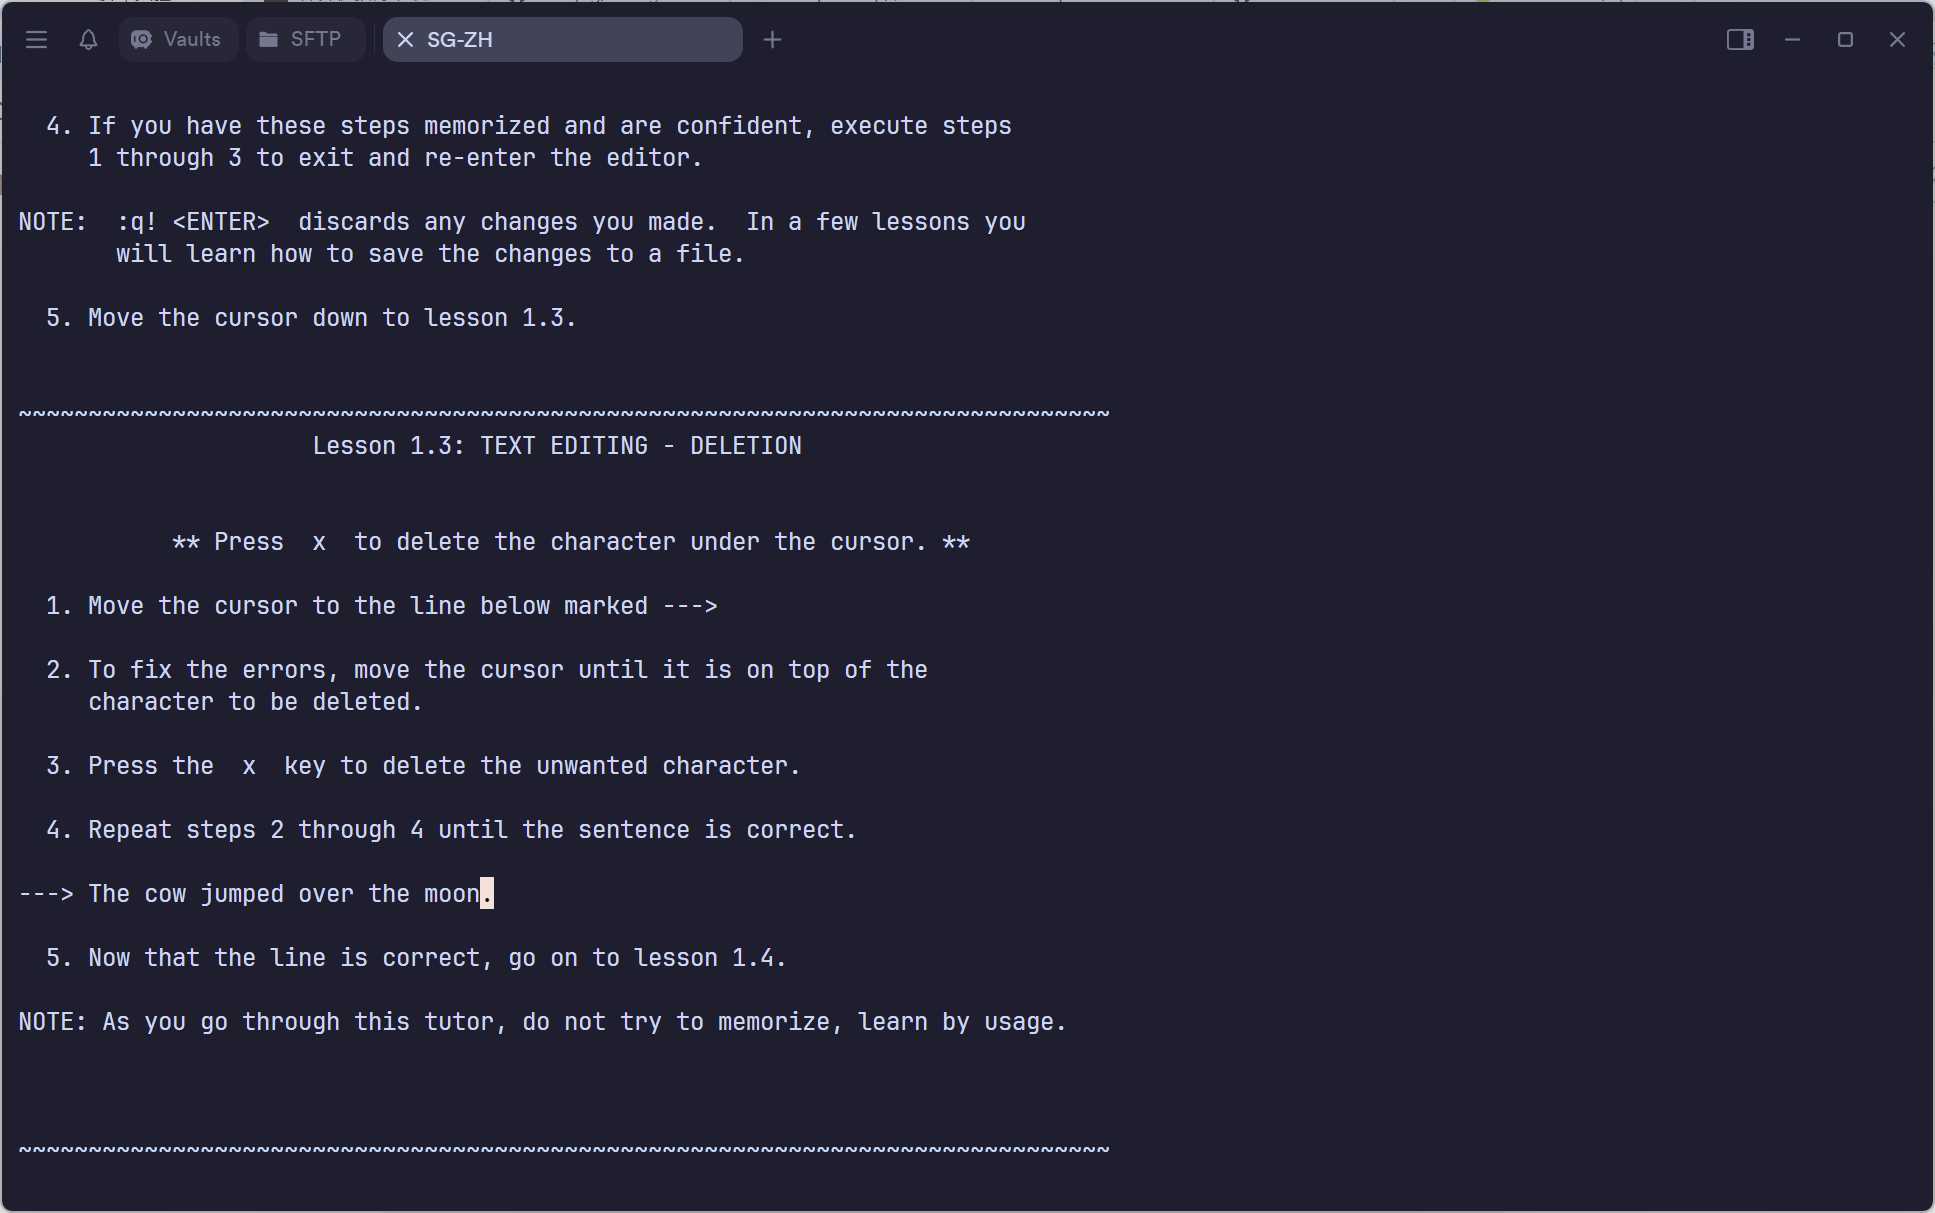
\includegraphics[width=0.9\textwidth]{Figures/vimtutor.png}
    \caption{Vimtutor学习}
    \label{fig:vimtutor}
\end{figure}